\documentclass[12pt, a4paper]{article}

\usepackage{graphicx}
\graphicspath{ {./img/} }
\usepackage[hidelinks]{hyperref}
\usepackage{amsmath}

\newcommand{\projectname}{Tutorial Time (TT)}

\setlength\parindent{0pt}

\usepackage{fancyhdr}
\setlength{\headheight}{15.2pt}
\pagestyle{fancy}
\fancyhf{}
\renewcommand{\headrulewidth}{0px}

\usepackage{tikz}
\usetikzlibrary{shapes.geometric, fit, positioning, backgrounds}

\fancyhead[L]{\projectname}
\fancyfoot[R]{\thepage}

\begin{document}

\pagenumbering{arabic}
\fancyfoot[R]{Page \thepage}

\section{Introduction}

This document describes the architecture overview of the project.
Based around the Clean Architecture and rooted in Domain-Driven Design, the aim is to make the project modular, maintainable and easy to extend or port.

\section{Clean Architecture}

As per the Clean Architecture, the following layers are present:

\begin{itemize}
\item \textbf{Domain}: the entities, data value objects and aggregates the project consists of;
\item \textbf{Use Cases}: the behaviors/uses of the objects in the domain layer;
\item \textbf{Adapters/Interfaces}: the interfaces used to decouple and connect the domain to the infrastructure;
\item \textbf{UI + Infrastructure}: a double-ended external layer, consisting of the user-facing web UI on one end, and the actual server infrastructure on the other.
\end{itemize}

\subsection{Diagram}

For the assignment, the following diagram was created:

\begin{center}

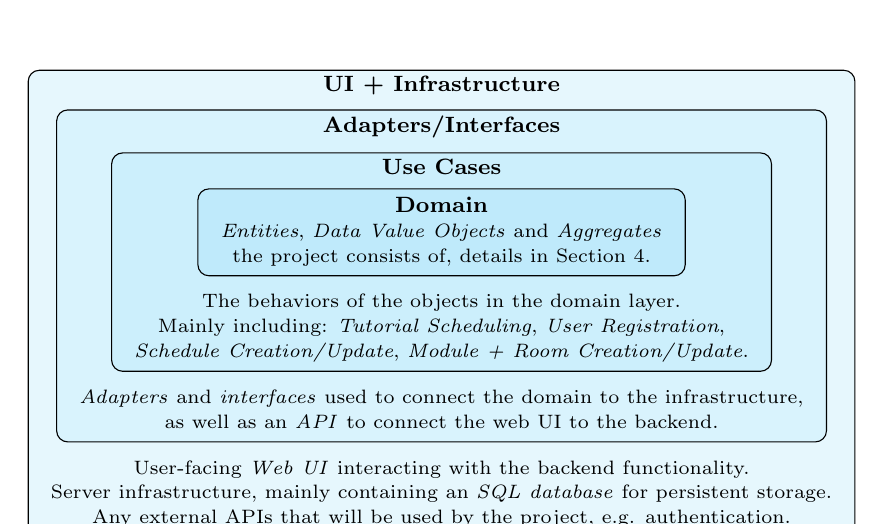
\begin{tikzpicture}[
            TextContainer/.style = {rectangle, inner sep = 0pt},
            FitContainer/.style args = {#1}{rectangle, rounded corners, inner sep = 2pt, draw, fit = #1}
        ]

    \renewcommand{\arraystretch}{0.75}

    \node(Domain) [TextContainer]
    {\begin{tabular}{c}
        \footnotesize \textbf{Domain} \\
        \scriptsize \emph{Entities}, \emph{Data Value Objects} and \emph{Aggregates} \\
        \scriptsize the project consists of, details in Section 4.
    \end{tabular}};

    \node(UseCasesTitle) [TextContainer, above = 2.5mm of Domain] {\footnotesize \textbf{Use Cases}};
    \node(AdaptersTitle) [TextContainer, above = 2.5mm of UseCasesTitle] {\footnotesize \textbf{Adapters/Interfaces}};
    \node(UITitle) [TextContainer, above = 2.5mm of AdaptersTitle] {\footnotesize \textbf{UI + Infrastructure}};

    \node(UseCases) [TextContainer, below = 2.5mm of Domain]
    {\begin{tabular}{c}
        \scriptsize The behaviors of the objects in the domain layer. \\
        \scriptsize Mainly including: \emph{Tutorial Scheduling}, \emph{User Registration}, \\ 
        \scriptsize \emph{Schedule Creation/Update}, \emph{Module + Room Creation/Update}.
    \end{tabular}};
    \node(Adapters) [TextContainer, below = 2.5mm of UseCases]
    {\begin{tabular}{c}
        \scriptsize \emph{Adapters} and \emph{interfaces} used to connect the domain to the infrastructure, \\
        \scriptsize as well as an \emph{API} to connect the web UI to the backend.
    \end{tabular}};
    \node(UI) [TextContainer, below = 2.5mm of Adapters]
    {\begin{tabular}{c}
        \scriptsize User-facing \emph{Web UI} interacting with the backend functionality. \\
        \scriptsize Server infrastructure, mainly containing an \emph{SQL database} for persistent storage. \\
        \scriptsize Any external APIs that will be used by the project, e.g. authentication.
    \end{tabular}};

    \begin{scope}[on background layer]
        \node [FitContainer=(Adapters) (UITitle) (UI), fill = cyan!10] {};
        \node [FitContainer=(UseCases) (AdaptersTitle) (Adapters), fill = cyan!15] {};
        \node [FitContainer=(Domain) (UseCasesTitle) (UseCases), fill = cyan!20] {};
        \node [FitContainer=(Domain), fill = cyan!25] {};
    \end{scope}

\end{tikzpicture}
\end{center}



\subsection{Domain}

The domain will contain the following entities:

\begin{itemize}
\item \textbf{Student}: identified by a university email (authentication) and student ID, containing a timetable/schedule;
\item \textbf{TA}: specific case of student, also identified by a university email/ID and containing a timetable/schedule;
\item \textbf{Lecturer}: identified by a university email and a staff ID, containing a timetable/schedule;
\item \textbf{Module}: identified by a module code, grouping students, lecturers and TAs together;
\item \textbf{Room}: identified by a room number, describing certain properties of rooms on campus (capacity, equipment etc.);
\item \textbf{Scheduler}: entity with a short life cycle associated with scheduling tutorial times, grouping together a module and a scheduler constraints data value object.
\end{itemize}

Along with this, the following data value objects will be present:

\begin{itemize}
\item \textbf{Timetable}: a filled out schedule of which timeslots in a week are free and which aren't;
\item \textbf{Room Properties}: any properties a room should have, like the capacity or equipment;
\item \textbf{Scheduler Constraints}: a set of constraints for a specific scheduler query.
\end{itemize}

This leaves us with the following aggregates:

\begin{itemize}
\item \textbf{Scheduler}: the aggregate root being a scheduler entity, this groups together a module and scheduler constraints;
\item \textbf{Student}: the aggregate root being the student ID, this groups together the student identity with a personal timetable;
\item \textbf{TA}: same as student, but with the inclusion of a specific identity as a TA;
\item \textbf{Lecturer}: the aggregate root being the staff ID, this groups together a lecturer identity with their personal timetable;
\item \textbf{Module}: the aggregate root is a module code, this groups a module identity to a list of students, TAs and lecturer;
\item \textbf{Room}: the aggregate root is the room number, associating a room identity with mutable properties, such as available equipment.
\end{itemize}

\subsection{Use Cases}

The use cases section focuses on behaviors and uses of the objects defined previously, in the domain layer.

The following are currently known/defined use cases:

\begin{itemize}
\item \textbf{Tutorial Scheduling}: taking in a Module and Scheduler Constraints, it should be possible to schedule appropriate tutorial slots;
\item \textbf{User Registration}: a new user should be able to authenticate with a university email, which will create a new entity if not already present;
\item \textbf{Schedule Creation}: an authenticated user should be able to fill in a timetable, which will then be associated with said user;
\item \textbf{Schedule Update}: an authenticated user should be able to fill in an updated timetable, which will replace an existing one;
\item \textbf{Module Creation}: a Lecturer can create a module given a module code and a list of student IDs;
\item \textbf{Room Registration}: in theory Buildings, in practice a Lecturer can fill out or update details of a room on campus, including any changes to available equipment.
\end{itemize}

\subsection{Adapters/Interfaces}

There are two primary directions of the described adapters and interfaces.
Firstly, there will be a repository system to interface with a data storage system, and secondly, interfaces providing backend API functionality will be present.

The data storage system interfaces are as follows:

\begin{itemize}
\item \textbf{User Repository}: saving and loading information about students, TAs and lecturers;
\item \textbf{Module Repository}: saving and loading information about modules;
\item \textbf{Room Repository}: saving and loading information about rooms.
\end{itemize}

Scheduler instances don't need a repository, as the scheduler lifecycle is short enough to not need persistent storage.

The backend API will be based around the following functions:

\begin{itemize}
\item \textbf{User Authentication}: authenticating a user;
\item \textbf{Schedule Read}: getting the schedule of the current user;
\item \textbf{Schedule Write}: setting the schedule of the current user;
\item \textbf{Module Creation}: associating a list of student IDs with a module code;
\item \textbf{Room Read}: getting information about a room;
\item \textbf{Room Write}: setting room details/information;
\item \textbf{Tutorial Scheduling}: getting tutorial slots given a module and constraints.
\end{itemize}

This API is subject to change based on further planning and development.

\subsection{UI + Infrastructure}

This section mostly implements the interfaces mentioned in the inner interface layer.
As mentioned, it's split between the web-based UI and the server-based infrastructure.

\subsubsection{Web UI}

The web UI will consist of frontend components, using the exposed API to interact with the software.

\subsubsection{Infrastructure}

The infrastructure will consist of specific implementations of the data storage interfaces.
This will include a specific (SQL-based) database technology, as well as any necessary general server functionality.

Optimally, this should be straightforward to implement a number of ways based on the available underlying infrastructure, which should make the application portable.

In addition, this layer also includes any external APIs used by the project, for example OAuth2 for user authentication.

\end{document}
